\documentclass{standalone}
\usepackage{tikz}
\usetikzlibrary{patterns, positioning}

\begin{document}
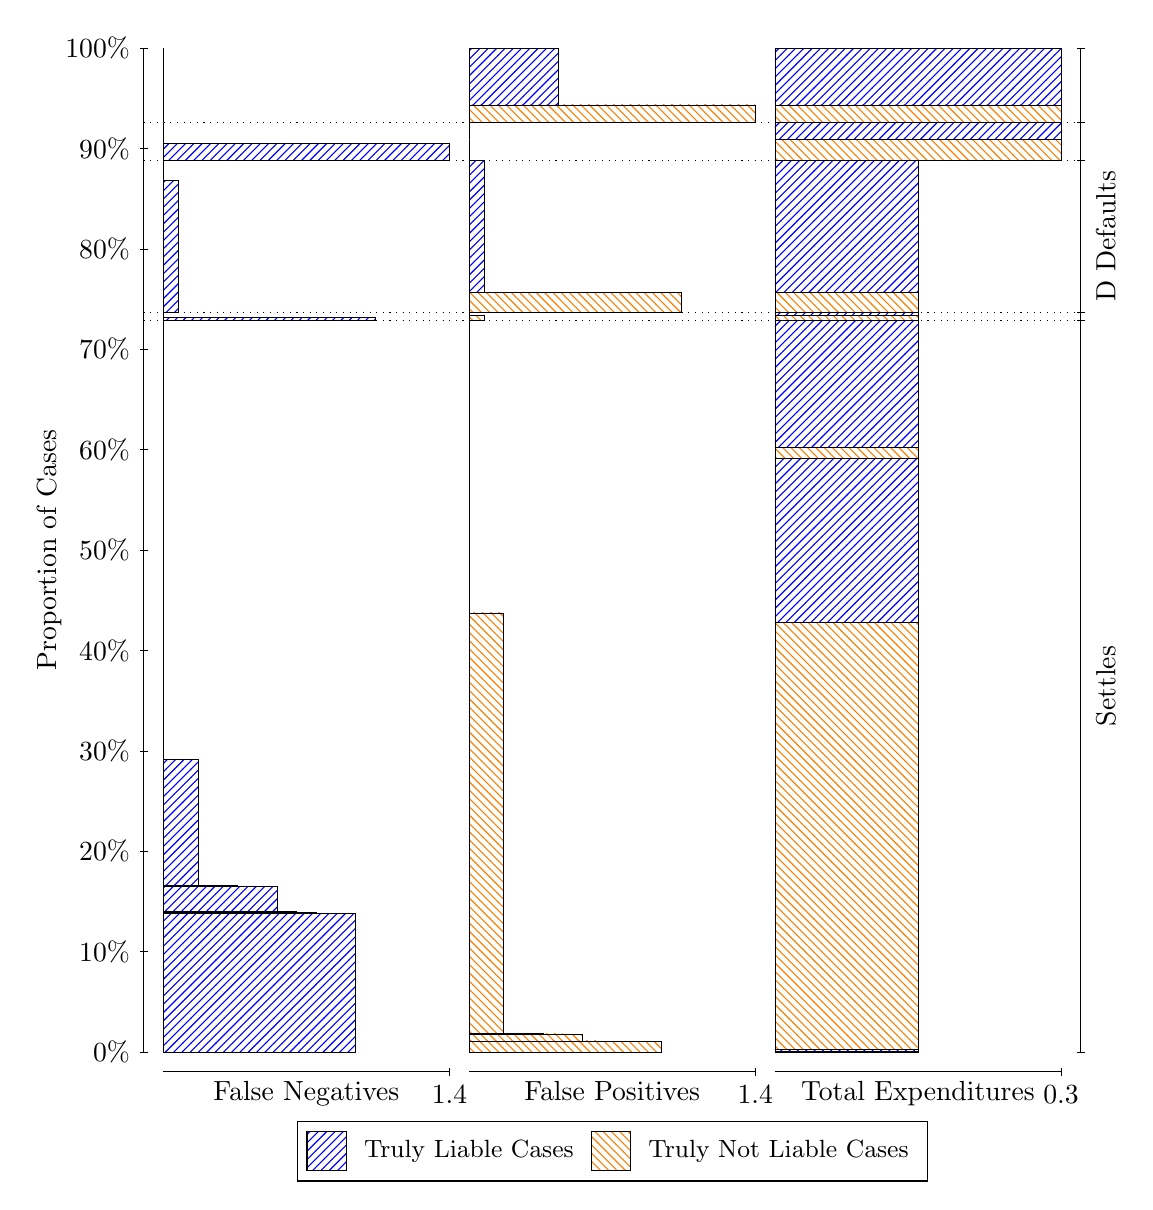
\begin{tikzpicture}
\draw[black, very thin] (1.5,1.75) -- (1.5,14.5);
\node[rotate=90, anchor=center] at (0.3, 8.125) {Proportion of Cases};
\draw[black, very thin] (1.45,1.75) -- (1.55,1.75);
\node[anchor=east] at (1.45, 1.75) {0\%};
\draw[black, very thin] (1.45,3.025) -- (1.55,3.025);
\node[anchor=east] at (1.45, 3.025) {10\%};
\draw[black, very thin] (1.45,4.3) -- (1.55,4.3);
\node[anchor=east] at (1.45, 4.3) {20\%};
\draw[black, very thin] (1.45,5.575) -- (1.55,5.575);
\node[anchor=east] at (1.45, 5.575) {30\%};
\draw[black, very thin] (1.45,6.85) -- (1.55,6.85);
\node[anchor=east] at (1.45, 6.85) {40\%};
\draw[black, very thin] (1.45,8.125) -- (1.55,8.125);
\node[anchor=east] at (1.45, 8.125) {50\%};
\draw[black, very thin] (1.45,9.4) -- (1.55,9.4);
\node[anchor=east] at (1.45, 9.4) {60\%};
\draw[black, very thin] (1.45,10.675) -- (1.55,10.675);
\node[anchor=east] at (1.45, 10.675) {70\%};
\draw[black, very thin] (1.45,11.95) -- (1.55,11.95);
\node[anchor=east] at (1.45, 11.95) {80\%};
\draw[black, very thin] (1.45,13.225) -- (1.55,13.225);
\node[anchor=east] at (1.45, 13.225) {90\%};
\draw[black, very thin] (1.45,14.5) -- (1.55,14.5);
\node[anchor=east] at (1.45, 14.5) {100\%};

\draw[black, very thin] (13.4,1.75) -- (13.4,14.5);
\draw[black, very thin] (13.35,1.75) -- (13.45,1.75);
\node[anchor=west] at (13.35, 1.75) {};
\draw[black, very thin] (13.35,11.043) -- (13.45,11.043);
\node[anchor=west] at (13.35, 11.043) {};
\draw[black, very thin] (13.35,11.141) -- (13.45,11.141);
\node[anchor=west] at (13.35, 11.141) {};
\draw[black, very thin] (13.35,13.072) -- (13.45,13.072);
\node[anchor=west] at (13.35, 13.072) {};
\draw[black, very thin] (13.35,13.556) -- (13.45,13.556);
\node[anchor=west] at (13.35, 13.556) {};
\draw[black, very thin] (13.35,14.5) -- (13.45,14.5);
\node[anchor=west] at (13.35, 14.5) {};

\draw[black, very thin, pattern color=blue, pattern=north east lines] (1.75,1.75) rectangle (4.1931,3.5073);
\draw[black, very thin, pattern color=blue, pattern=north east lines] (1.75,3.5073) rectangle (3.9425,3.5147);
\draw[black, very thin, pattern color=blue, pattern=north east lines] (1.75,3.5147) rectangle (3.692,3.5227);
\draw[black, very thin, pattern color=blue, pattern=north east lines] (1.75,3.5227) rectangle (3.4414,3.5316);
\draw[black, very thin, pattern color=blue, pattern=north east lines] (1.75,3.5316) rectangle (3.1908,3.8542);
\draw[black, very thin, pattern color=blue, pattern=north east lines] (1.75,3.8542) rectangle (2.9402,3.8574);
\draw[black, very thin, pattern color=blue, pattern=north east lines] (1.75,3.8574) rectangle (2.6897,3.8608);
\draw[black, very thin, pattern color=blue, pattern=north east lines] (1.75,3.8608) rectangle (2.4391,3.8642);
\draw[black, very thin, pattern color=blue, pattern=north east lines] (1.75,3.8642) rectangle (2.1885,5.4679);
\draw[black, very thin, pattern color=orange, pattern=north west lines] (1.75,5.4679) rectangle (1.75,11.043);
\draw[black, very thin, pattern color=blue, pattern=north east lines] (1.75,11.043) rectangle (4.4437,11.083);
\draw[black, very thin, pattern color=orange, pattern=north west lines] (1.75,11.083) rectangle (1.75,11.141);
\draw[black, very thin, pattern color=blue, pattern=north east lines] (1.75,11.141) rectangle (1.9379,12.815);
\draw[black, very thin, pattern color=orange, pattern=north west lines] (1.75,12.815) rectangle (1.75,13.072);
\draw[black, very thin, pattern color=blue, pattern=north east lines] (1.75,13.072) rectangle (5.3833,13.293);
\draw[black, very thin, pattern color=orange, pattern=north west lines] (1.75,13.293) rectangle (1.75,13.556);
\draw[black, very thin, pattern color=orange, pattern=north west lines] (1.75,13.556) rectangle (1.75,13.778);
\draw[black, very thin, pattern color=blue, pattern=north east lines] (1.75,13.778) rectangle (1.75,14.5);
\draw[black, very thin, pattern color=orange, pattern=north west lines] (5.6333,1.75) rectangle (8.0764,1.8875);
\draw[black, very thin, pattern color=orange, pattern=north west lines] (5.6333,1.8875) rectangle (7.8259,1.8882);
\draw[black, very thin, pattern color=orange, pattern=north west lines] (5.6333,1.8882) rectangle (7.5753,1.8889);
\draw[black, very thin, pattern color=orange, pattern=north west lines] (5.6333,1.8889) rectangle (7.3247,1.8896);
\draw[black, very thin, pattern color=orange, pattern=north west lines] (5.6333,1.8896) rectangle (7.0741,1.9777);
\draw[black, very thin, pattern color=orange, pattern=north west lines] (5.6333,1.9777) rectangle (6.8236,1.9777);
\draw[black, very thin, pattern color=orange, pattern=north west lines] (5.6333,1.9777) rectangle (6.8236,1.9801);
\draw[black, very thin, pattern color=orange, pattern=north west lines] (5.6333,1.9801) rectangle (6.573,1.9823);
\draw[black, very thin, pattern color=orange, pattern=north west lines] (5.6333,1.9823) rectangle (6.3224,1.9843);
\draw[black, very thin, pattern color=orange, pattern=north west lines] (5.6333,1.9843) rectangle (6.0718,7.325);
\draw[black, very thin, pattern color=blue, pattern=north east lines] (5.6333,7.325) rectangle (5.6333,11.043);
\draw[black, very thin, pattern color=orange, pattern=north west lines] (5.6333,11.043) rectangle (5.8213,11.1);
\draw[black, very thin, pattern color=blue, pattern=north east lines] (5.6333,11.1) rectangle (5.6333,11.141);
\draw[black, very thin, pattern color=orange, pattern=north west lines] (5.6333,11.141) rectangle (8.327,11.398);
\draw[black, very thin, pattern color=blue, pattern=north east lines] (5.6333,11.398) rectangle (5.8213,13.072);
\draw[black, very thin, pattern color=orange, pattern=north west lines] (5.6333,13.072) rectangle (5.6333,13.336);
\draw[black, very thin, pattern color=blue, pattern=north east lines] (5.6333,13.336) rectangle (5.6333,13.556);
\draw[black, very thin, pattern color=orange, pattern=north west lines] (5.6333,13.556) rectangle (9.2667,13.778);
\draw[black, very thin, pattern color=blue, pattern=north east lines] (5.6333,13.778) rectangle (6.7609,14.5);
\draw[black, very thin, pattern color=orange, pattern=north west lines] (9.5167,1.75) rectangle (11.333,1.7566);
\draw[black, very thin, pattern color=blue, pattern=north east lines] (9.5167,1.7566) rectangle (11.333,1.781);
\draw[black, very thin, pattern color=orange, pattern=north west lines] (9.5167,1.781) rectangle (11.333,7.2098);
\draw[black, very thin, pattern color=blue, pattern=north east lines] (9.5167,7.2098) rectangle (11.333,9.2896);
\draw[black, very thin, pattern color=orange, pattern=north west lines] (9.5167,9.2896) rectangle (11.333,9.4293);
\draw[black, very thin, pattern color=blue, pattern=north east lines] (9.5167,9.4293) rectangle (11.333,11.043);
\draw[black, very thin, pattern color=orange, pattern=north west lines] (9.5167,11.043) rectangle (11.333,11.1);
\draw[black, very thin, pattern color=blue, pattern=north east lines] (9.5167,11.1) rectangle (11.333,11.141);
\draw[black, very thin, pattern color=orange, pattern=north west lines] (9.5167,11.141) rectangle (11.333,11.398);
\draw[black, very thin, pattern color=blue, pattern=north east lines] (9.5167,11.398) rectangle (11.333,13.072);
\draw[black, very thin, pattern color=orange, pattern=north west lines] (9.5167,13.072) rectangle (13.15,13.336);
\draw[black, very thin, pattern color=blue, pattern=north east lines] (9.5167,13.336) rectangle (13.15,13.556);
\draw[black, very thin, pattern color=orange, pattern=north west lines] (9.5167,13.556) rectangle (13.15,13.778);
\draw[black, very thin, pattern color=blue, pattern=north east lines] (9.5167,13.778) rectangle (13.15,14.5);
\draw[black, dotted] (1.5,11.043) -- (13.4,11.043);
\draw[black, dotted] (1.5,11.141) -- (13.4,11.141);
\draw[black, dotted] (1.5,13.072) -- (13.4,13.072);
\draw[black, dotted] (1.5,13.556) -- (13.4,13.556);
\draw[black, very thin] (1.75,1.5) -- (5.3833,1.5);
\node[anchor=north] at (3.5667, 1.5) {False Negatives};
\draw[black, very thin] (5.3833,1.45) -- (5.3833,1.55);
\node[anchor=north] at (5.3833, 1.45) {1.4};

\draw[black, very thin] (5.6333,1.5) -- (9.2667,1.5);
\node[anchor=north] at (7.45, 1.5) {False Positives};
\draw[black, very thin] (9.2667,1.45) -- (9.2667,1.55);
\node[anchor=north] at (9.2667, 1.45) {1.4};

\draw[black, very thin] (9.5167,1.5) -- (13.15,1.5);
\node[anchor=north] at (11.333, 1.5) {Total Expenditures};
\draw[black, very thin] (13.15,1.45) -- (13.15,1.55);
\node[anchor=north] at (13.15, 1.45) {0.3};

\node[black, centered, rotate=90] at (13.72, 6.3965) {Settles};

\node[black, centered, rotate=90] at (13.72, 12.107) {D Defaults};



\draw (7.449999999999999,1.5) node[draw=none] (baseCoordinate) {};
\begin{scope}[align=center]
        \matrix[scale=0.5, draw=black, below=0.5cm of baseCoordinate, nodes={draw}, column sep=0.1cm]{
            \node[rectangle, draw, minimum width=0.5cm, minimum height=0.5cm, pattern=north east lines, pattern color=blue] {}; &
            \node[draw=none, font=\small] (B) {Truly Liable Cases}; &
            \node[rectangle, draw, minimum width=0.5cm, minimum height=0.5cm, pattern=north west lines, pattern color=orange] {}; &
            \node[draw=none, font=\small] (B) {Truly Not Liable Cases}; \\
            };
\end{scope}

\end{tikzpicture}
\end{document}